% !TeX program = xelatex
\documentclass[a4paper,10pt]{article}

% ============================================================================
% កញ្ចប់បណ្ណាល័យ (Packages) – តាមលំនាំ NGS Preah Krasang (ls_plan.tex)
% ============================================================================
\usepackage[a4paper, left=0.95cm, right=0.95cm, top=0.85cm, bottom=0.92cm, footskip=0.52cm]{geometry}
\usepackage{amsmath}
\usepackage{unicode-math}
\usepackage{fontspec}
\usepackage{array, longtable, multirow, colortbl}
\usepackage[table]{xcolor}
\usepackage{enumitem}
\usepackage{pifont}
\usepackage{fancyhdr}
\usepackage{tikz}
\usetikzlibrary{calc, arrows.meta, angles, quotes, decorations.markings, babel}

% LaTeX 2025 + longtable v4.24 compatibility guard
\makeatletter
\let\@expl@@@mark@update@singlecol@structures@@\relax
\makeatother

% ============================================================================
% ការកំណត់ពុម្ពអក្សរ (Fonts Configuration) – តាមលំនាំស្ដង់ដារ ១០០%
% ============================================================================
% Cross-platform font path resolver (Windows local + Linux/Cloud repo fonts/)
\providecommand{\NGSFindFonts}{%
  \IfFileExists{C:/Windows/Fonts/cambria.ttc}{%
    \def\NGSSysPath{C:/Windows/Fonts/}%
    \def\NGSUserPath{C:/Users/KIT/AppData/Local/Microsoft/Windows/Fonts/}%
  }{%
    \IfFileExists{./fonts/KhmerOSsiemreap.ttf}{\def\NGSSysPath{./fonts/}\def\NGSUserPath{./fonts/}}{%
    \IfFileExists{../fonts/KhmerOSsiemreap.ttf}{\def\NGSSysPath{../fonts/}\def\NGSUserPath{../fonts/}}{%
    \IfFileExists{../../fonts/KhmerOSsiemreap.ttf}{\def\NGSSysPath{../../fonts/}\def\NGSUserPath{../../fonts/}}{%
    \IfFileExists{../../../fonts/KhmerOSsiemreap.ttf}{\def\NGSSysPath{../../../fonts/}\def\NGSUserPath{../../../fonts/}}{%
    \IfFileExists{../../../../fonts/KhmerOSsiemreap.ttf}{\def\NGSSysPath{../../../../fonts/}\def\NGSUserPath{../../../../fonts/}}{%
    \IfFileExists{../../../../../fonts/KhmerOSsiemreap.ttf}{\def\NGSSysPath{../../../../../fonts/}\def\NGSUserPath{../../../../../fonts/}}{%
    \IfFileExists{../../../../../../fonts/KhmerOSsiemreap.ttf}{\def\NGSSysPath{../../../../../../fonts/}\def\NGSUserPath{../../../../../../fonts/}}{%
      \def\NGSSysPath{../../../../../../../fonts/}\def\NGSUserPath{../../../../../../../fonts/}%
    }}}}}}}%
  }%
}
\NGSFindFonts

\setmathfont[
  Path={\NGSSysPath},
  FontIndex=1,
  Scale=1.02
]{cambria.ttc}

\defaultfontfeatures{Ligatures=TeX}

\setmainfont[
  Path={\NGSUserPath},
  Extension=.ttf,
  Script=Khmer,
  BoldFont={KhmerOSsiemreap},
  BoldFeatures={FakeBold=1.8},
  ItalicFont={KhmerOSsiemreap},
  ItalicFeatures={FakeSlant=0.25},
  BoldItalicFont={KhmerOSsiemreap},
  BoldItalicFeatures={FakeBold=1.8, FakeSlant=0.25}
]{KhmerOSsiemreap}

\newfontfamily\muol[
  Path={\NGSUserPath},
  Extension=.ttf,
  Script=Khmer
]{KhmerOSmuollight}

\newfontfamily\TimesEn[
  Path={\NGSSysPath},
  Extension=.ttf,
  Scale=1.00,
  BoldFont={timesbd},
  ItalicFont={timesi},
  BoldItalicFont={timesbi}
]{times}

\newfontfamily\NagaBold[
  Path={\NGSUserPath},
  Extension=.ttf
]{AKbalthom Naga Bold}

\newfontfamily\CalibriFont[
  Path={\NGSSysPath},
  Extension=.ttf
]{calibri}

\newfontfamily\Tacteing[
  Path={\NGSUserPath}
]{TACTENG.TTF}

\newfontfamily\CourierBullet[
  Path={\NGSSysPath},
  Extension=.ttf
]{cour}
\newcommand{\wcirc}{{\CourierBullet\fontsize{9.5pt}{11pt}\selectfont o}}

% ក្បួនកាត់ពាក្យខ្មែរ (Khmer word wrapping)
\XeTeXlinebreaklocale "km"
\XeTeXlinebreakskip = 0pt plus 1pt minus 0.1pt

% ============================================================================
% ការកំណត់ពណ៌ និងទម្រង់ទំព័រ (Colors & Page Style)
% ============================================================================
\definecolor{stepgray}{HTML}{D9D9D9}
\definecolor{headgray}{HTML}{F2F2F2}
\definecolor{boxgray}{HTML}{D9D9D9}
\definecolor{darkred}{HTML}{C00000}
\definecolor{red5e}{HTML}{FF0000}

\pagestyle{fancy}
\fancyhf{}
\renewcommand{\headrulewidth}{0pt}
\fancyfoot[R]{\CalibriFont\fontsize{11pt}{13pt}\selectfont\thepage}

\setlength{\parindent}{0pt}
\setlength{\parskip}{0pt}
\setlength{\tabcolsep}{3.8pt}

\newcolumntype{L}[1]{>{\raggedright\arraybackslash}p{#1}}

% ============================================================================
% ម៉ាក្រូជំនួយ (Helper Macros)
% ============================================================================
\newcommand{\en}[1]{{\TimesEn #1}}
\newcommand{\enbf}[1]{{\TimesEn\textbf{#1}}}
\newcommand{\fiveE}[1]{{\NagaBold\fontsize{9.5pt}{13pt}\selectfont\textcolor{red5e}{#1}}}
\newcommand{\timenote}[1]{\textcolor{darkred}{\textit{#1}}}
\newcommand{\redsub}[1]{\textcolor{darkred}{#1}}
\newcommand{\graybox}[1]{\colorbox{boxgray}{\strut\hspace{2pt}#1\hspace{2pt}}}
\newcommand{\ditem}{\tikz[baseline=-0.5ex]\fill (0,0.42ex) -- (0.42ex,0) -- (0,-0.42ex) -- (-0.42ex,0) -- cycle;\hspace{0.3em}}
\newcommand{\cnum}[1]{{\fontsize{10.5pt}{12pt}\selectfont\ding{\numexpr181+#1\relax}}\hspace{0.2em}}
\newcommand{\cfig}[1]{\par\vspace{4pt}{\centering #1\par}\vspace{4pt}}
\newcommand{\stepheader}[1]{\multicolumn{3}{|c|}{\cellcolor{stepgray}\muol #1} \\* \noalign{\hrule height 0.4pt}}
\newcommand{\tri}[1]{\ensuremath{\triangle #1}}
\newcommand{\ang}[1]{\ensuremath{\angle #1}}
\newcommand{\cg}{\ensuremath{\cong}}
\newcommand{\ncg}{\ensuremath{\not\cong}}

% រចនាប័ទ្មគូសសម្គាល់ជ្រុងស្មើគ្នា (Tick mark styles - bold B&W print safe)
\tikzset{
  tk1/.style={postaction={decorate},decoration={markings,mark=at position 0.50 with {\draw[black, line width=0.85pt](0,-0.095)--(0,0.095);}}},
  tk1a/.style={postaction={decorate},decoration={markings,mark=at position 0.30 with {\draw[black, line width=0.85pt](0,-0.095)--(0,0.095);}}},
  tk2/.style={postaction={decorate},decoration={markings,
    mark=at position 0.45 with {\draw[black, line width=0.85pt](0,-0.095)--(0,0.095);},
    mark=at position 0.55 with {\draw[black, line width=0.85pt](0,-0.095)--(0,0.095);}}},
  hypArrow/.style={black, densely dashed, line width=0.8pt, -{Stealth[length=3.5pt]}}
}

% ម៉ាក្រូគូសប្រអប់មុំកែង 90° ត្រង់ B ក្នុងមុំ A-B-C
\newcommand{\rightbox}[4][0.19]{%
  \draw[black, line width=0.8pt]
    ($(#3)!#1!(#2)$) -- ($($(#3)!#1!(#2)$)+($(#3)!#1!(#4)$)-(#3)$) -- ($(#3)!#1!(#4)$);
}

% ក្បាច់ក្រោមបាវចនា (Tacteing Font - Keyboard '3')
\newcommand{\khmflourish}{{\Tacteing\fontsize{36pt}{14pt}\selectfont\raisebox{-5pt}{3}}}

% ============================================================================
% ម៉ាក្រូគូសរូបធរណីមាត្រ (Monochrome B&W TikZ Figures, 100% Black Text)
% ============================================================================

% ១. កំណែកិច្ចការផ្ទះមេរៀនមុន (លំហាត់ #6 ទំ.១៦៤ & #7 ទំ.១៦៥)
\newcommand{\figHWoldHL}{%
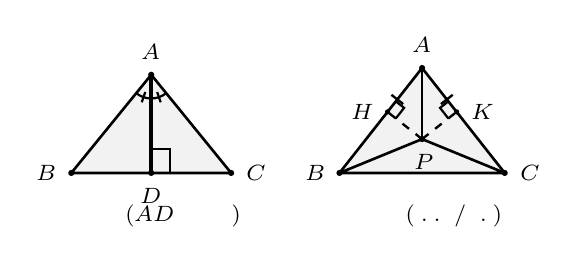
\begin{tikzpicture}[scale=0.86, every node/.style={font=\footnotesize, text=black}]
  % លំហាត់ទី៦ (AD ជាជ្រុងមុំកែងរួម, ម.ជ.ម)
  \begin{scope}[shift={(-2.05,0)}]
    \coordinate (A) at (0, 1.45);
    \coordinate (B) at (-1.18, 0);
    \coordinate (C) at (1.18, 0);
    \coordinate (D) at (0, 0);
    \fill[gray!10] (A) -- (B) -- (C) -- cycle;
    \draw[black, line width=0.95pt] (A) -- (B) -- (C) -- cycle;
    \draw[black, line width=1.25pt] (A) -- (D);
    \rightbox[0.24]{A}{D}{C}
    \draw[black, line width=0.8pt] ($(A)+(-129:0.35)$) arc (-129:-51:0.35);
    \draw[black, line width=0.8pt] ($(A)+(-109:0.27)$) -- ($(A)+(-109:0.43)$);
    \draw[black, line width=0.8pt] ($(A)+(-71:0.27)$) -- ($(A)+(-71:0.43)$);
    \fill[black] (A) circle (1.3pt) node[above=2pt] {$A$};
    \fill[black] (B) circle (1.3pt) node[left=2pt] {$B$};
    \fill[black] (C) circle (1.3pt) node[right=2pt] {$C$};
    \fill[black] (D) circle (1.3pt) node[below=2pt] {$D$};
    \node[anchor=north] at (0,-0.32) {លំហាត់ទី៦ ($AD$ ជ្រុងកែង)};
  \end{scope}
  % លំហាត់ទី៧ (P លើពុះមុំ A, ក. PB=PC, ខ. PH⊥AB, PK⊥AC)
  \begin{scope}[shift={(1.95,0)}]
    \coordinate (A) at (0, 1.55);
    \coordinate (B) at (-1.22, 0);
    \coordinate (C) at (1.22, 0);
    \coordinate (P) at (0, 0.50);
    \coordinate (H) at ($(A)!(P)!(B)$);
    \coordinate (K) at ($(A)!(P)!(C)$);
    \fill[gray!10] (A) -- (B) -- (C) -- cycle;
    \draw[black, line width=0.95pt, tk1a] (A) -- (B);
    \draw[black, line width=0.95pt, tk1a] (A) -- (C);
    \draw[black, line width=0.95pt] (B) -- (C) (B) -- (P) -- (C);
    \draw[black, line width=0.9pt] (A) -- (P);
    \draw[black, line width=0.85pt, dashed] (P) -- (H) (P) -- (K);
    \rightbox[0.24]{P}{H}{A}
    \rightbox[0.24]{P}{K}{A}
    \fill[black] (A) circle (1.3pt) node[above=2pt] {$A$};
    \fill[black] (B) circle (1.3pt) node[left=2pt] {$B$};
    \fill[black] (C) circle (1.3pt) node[right=2pt] {$C$};
    \fill[black] (P) circle (1.3pt) node[below=2pt] {$P$};
    \fill[black] (H) circle (1.1pt) node[left=2pt] {$H$};
    \fill[black] (K) circle (1.1pt) node[right=2pt] {$K$};
    \node[anchor=north] at (0,-0.32) {លំហាត់ទី៧ (ជ.ម.ជ / អ.ម)};
  \end{scope}
\end{tikzpicture}}

% ២. រំលឹកទី១៖ មុំរាប 180° & △BCB' សមបាទ (∠B=∠B') + លក្ខខណ្ឌ អ.ម & ពុះមុំ
\newcommand{\figPrereqHL}{%
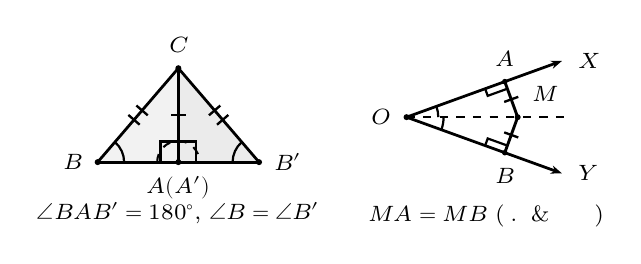
\begin{tikzpicture}[scale=0.84, every node/.style={font=\footnotesize, text=black}]
  % ឆ្វេង៖ មុំរាប 90° + 90° = 180° និង △BCB' សមបាទ
  \begin{scope}[shift={(-2.10,0)}]
    \coordinate (A) at (0,0);
    \coordinate (C) at (0,1.42);
    \coordinate (B) at (-1.22,0);
    \coordinate (Bp) at (1.22,0);
    \fill[gray!10] (B) -- (C) -- (A) -- cycle;
    \fill[gray!16] (A) -- (C) -- (Bp) -- cycle;
    \draw[black, line width=1.05pt] (B) -- (Bp);
    \draw[black, line width=1.0pt, tk1] (A) -- (C);
    \draw[black, line width=1.0pt, tk2] (C) -- (B);
    \draw[black, line width=1.0pt, tk2] (C) -- (Bp);
    \rightbox[0.22]{C}{A}{B}
    \rightbox[0.22]{C}{A}{Bp}
    \draw[black, line width=0.8pt] (-0.82,0) arc (0:49:0.40);
    \draw[black, line width=0.8pt] (0.82,0) arc (180:131:0.40);
    \draw[black, line width=0.75pt, dashed] (-0.32,0) arc (180:0:0.32);
    \fill[black] (A) circle (1.3pt) node[below=1.5pt] {$A(A')$};
    \fill[black] (C) circle (1.3pt) node[above=2pt] {$C$};
    \fill[black] (B) circle (1.3pt) node[left=2pt] {$B$};
    \fill[black] (Bp) circle (1.3pt) node[right=2pt] {$B'$};
    \node[anchor=north] at (0,-0.46) {$\ang{BAB'}=180^\circ,\, \ang{B}=\ang{B'}$};
  \end{scope}
  % ស្ដាំ៖ រំលឹក អ.ម & ពុះមុំ MA=MB
  \begin{scope}[shift={(1.35,0.68)}]
    \coordinate (O) at (0,0);
    \coordinate (X) at (2.35, 0.85);
    \coordinate (Y) at (2.35, -0.85);
    \coordinate (M) at (1.68, 0);
    \coordinate (A) at ($(O)!(M)!(X)$);
    \coordinate (B) at ($(O)!(M)!(Y)$);
    \draw[black, line width=1.0pt, -{Stealth[length=4pt]}] (O) -- (X) node[right=2pt] {$X$};
    \draw[black, line width=1.0pt, -{Stealth[length=4pt]}] (O) -- (Y) node[right=2pt] {$Y$};
    \draw[black, line width=0.85pt, dashed] (O) -- (2.45,0);
    \draw[black, line width=1.05pt, tk1] (M) -- (A);
    \draw[black, line width=1.05pt, tk1] (M) -- (B);
    \rightbox[0.20]{M}{A}{O}
    \rightbox[0.20]{M}{B}{O}
    \draw[black, line width=0.8pt] (0.48,0) arc (0:20:0.48);
    \draw[black, line width=0.8pt] (0.56,0) arc (0:-20:0.56);
    \fill[black] (O) circle (1.3pt) node[left=2pt] {$O$};
    \fill[black] (M) circle (1.3pt) node[above right=2pt] {$M$};
    \fill[black] (A) circle (1.2pt) node[above=2pt] {$A$};
    \fill[black] (B) circle (1.2pt) node[below=2pt] {$B$};
    \node[below=8pt] at (1.20,-0.84) {$MA=MB$ (អ.ម \& ពុះមុំ)};
  \end{scope}
\end{tikzpicture}}

% ៣. E1 Engage: អាងទឹករង្វង់សួនផ្លូវប្រសព្វ ៣ ខ្សែ (Scalene △ABC + រង្វង់ចារឹកក្នុង)
\newcommand{\figEngageHL}{%
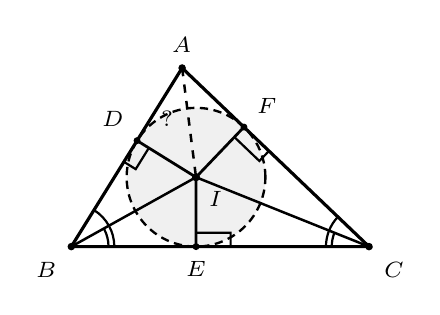
\begin{tikzpicture}[scale=1.05, every node/.style={font=\footnotesize, text=black}]
  \coordinate (B) at (0,0);
  \coordinate (C) at (3.60,0);
  \coordinate (A) at (1.34,2.16);
  \coordinate (I) at (1.508,0.839);
  \coordinate (D) at ($(B)!(I)!(A)$);
  \coordinate (E) at ($(B)!(I)!(C)$);
  \coordinate (F) at ($(A)!(I)!(C)$);
  \fill[gray!12] (I) circle (0.839);
  \draw[black, line width=0.85pt, densely dashed] (I) circle (0.839);
  \draw[black, line width=1.15pt] (A) -- (B) -- (C) -- cycle;
  \draw[black, line width=0.9pt] (B) -- (I) (C) -- (I);
  \draw[black, line width=0.9pt, dashed] (A) -- (I);
  \draw[black, line width=1.0pt] (I) -- (D) (I) -- (E) (I) -- (F);
  \rightbox[0.20]{I}{D}{B}
  \rightbox[0.20]{I}{E}{C}
  \rightbox[0.20]{I}{F}{C}
  \draw[black, line width=0.8pt] (0.45,0) arc (0:29:0.45);
  \draw[black, line width=0.8pt] (0.52,0) arc (0:58:0.52);
  \draw[black, line width=0.8pt] (3.15,0) arc (180:158:0.45);
  \draw[black, line width=0.8pt] (3.08,0) arc (180:136:0.52);
  \node[left=2pt] at (1.42,1.55) {$?$};
  \fill[black] (A) circle (1.3pt) node[above=2pt] {$A$};
  \fill[black] (B) circle (1.3pt) node[below left=2pt] {$B$};
  \fill[black] (C) circle (1.3pt) node[below right=2pt] {$C$};
  \fill[black] (I) circle (1.4pt) node[below right=1.5pt] {$I$};
  \fill[black] (D) circle (1.2pt) node[above left=1.5pt] {$D$};
  \fill[black] (E) circle (1.2pt) node[below=2pt] {$E$};
  \fill[black] (F) circle (1.2pt) node[above right=1.5pt] {$F$};
\end{tikzpicture}}

% ៤. E2 Act 1: 3-4-5 cm ត្រឡប់ខ្នងគ្នា (∠BAB'=180°) vs អន្ទាក់ 35° SSA កាត់ ២ ដង
\newcommand{\figExploreOneHL}{%
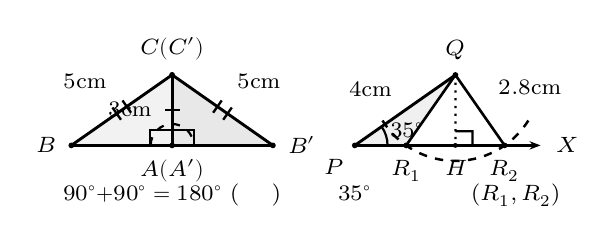
\begin{tikzpicture}[scale=0.80, every node/.style={font=\footnotesize, text=black}]
  % ឆ្វេង៖ 3-4-5 cm ត្រឡប់ខ្នងគ្នា AC=A'C'=3cm, BC=B'C'=5cm
  \begin{scope}[shift={(0,0)}]
    \coordinate (A) at (0,0);
    \coordinate (C) at (0,1.12);
    \coordinate (B) at (-1.60,0);
    \coordinate (Bp) at (1.60,0);
    \fill[gray!10] (B) -- (C) -- (A) -- cycle;
    \fill[gray!18] (A) -- (C) -- (Bp) -- cycle;
    \draw[black, line width=1.05pt] (B) -- (Bp);
    \draw[black, line width=1.05pt, tk1] (A) -- (C);
    \draw[black, line width=1.05pt, tk2] (C) -- (B);
    \draw[black, line width=1.05pt, tk2] (C) -- (Bp);
    \rightbox[0.22]{C}{A}{B}
    \rightbox[0.22]{C}{A}{Bp}
    \draw[black, line width=0.8pt, dashed] (-0.34,0) arc (180:0:0.34);
    \node[above left=1.5pt] at (-0.82,0.68) {$5\text{cm}$};
    \node[above right=1.5pt] at (0.82,0.68) {$5\text{cm}$};
    \node[left=3pt] at (-0.04,0.58) {$3\text{cm}$};
    \fill[black] (A) circle (1.3pt) node[below=1.5pt] {$A(A')$};
    \fill[black] (C) circle (1.3pt) node[above=2pt] {$C(C')$};
    \fill[black] (B) circle (1.3pt) node[left=2pt] {$B$};
    \fill[black] (Bp) circle (1.3pt) node[right=2pt] {$B'$};
    \node[anchor=north] at (0,-0.46) {$90^\circ{+}90^\circ=180^\circ$ (១ គត់)};
  \end{scope}
  % ស្ដាំ៖ មុំស្រួច 35° (PQ=4cm, កាំ r=2.8cm កាត់ 2 ដង R1, R2 vs H)
  \begin{scope}[shift={(2.90,0)}]
    \coordinate (P) at (0,0);
    \coordinate (X) at (2.95,0);
    \coordinate (Q) at (35:1.95);
    \coordinate (H) at (1.597,0);
    \coordinate (R1) at (0.816,0);
    \coordinate (R2) at (2.378,0);
    \fill[gray!12] (P) -- (Q) -- (R1) -- cycle;
    \draw[black, line width=1.0pt, -{Stealth[length=4pt]}] (P) -- (X) node[right=2pt] {$X$};
    \draw[black, line width=1.05pt] (P) -- (Q) node[midway, above left=1pt] {$4\text{cm}$};
    \draw[black, line width=0.95pt] (Q) -- (R1) (Q) -- (R2);
    \draw[black, line width=0.8pt, dotted] (Q) -- (H);
    \rightbox[0.20]{Q}{H}{X}
    \draw[black, line width=0.9pt, dashed] ($(Q)+(-148:1.365)$) arc (-148:-32:1.365);
    \draw[black, line width=0.8pt] (0.52,0) arc (0:35:0.52);
    \node at (16:0.86) {$35^\circ$};
    \node[above right=1.5pt] at (2.06,0.58) {$2.8\text{cm}$};
    \fill[black] (P) circle (1.3pt) node[below left=1.5pt] {$P$};
    \fill[black] (Q) circle (1.3pt) node[above=2pt] {$Q$};
    \fill[black] (R1) circle (1.3pt) node[below=2pt] {$R_1$};
    \fill[black] (R2) circle (1.3pt) node[below=2pt] {$R_2$};
    \fill[black] (H) circle (1.1pt) node[below=2pt] {$H$};
    \node[anchor=north] at (1.50,-0.46) {$35^\circ$ កាត់ ២ កន្លែង ($R_1, R_2$)};
  \end{scope}
\end{tikzpicture}}

% ៥. E2 Act 2 POE: បត់ក្រដាស scalene △ABC (9.2-6.5-8.0 cm) រកផ្ចិត I & រង្វង់ចារឹកក្នុង
\newcommand{\figExploreTwoHL}{%
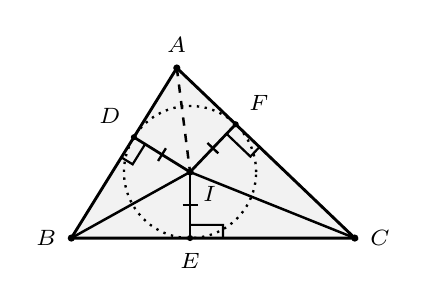
\begin{tikzpicture}[scale=1.00, every node/.style={font=\footnotesize, text=black}]
  \coordinate (B) at (0,0);
  \coordinate (C) at (3.60,0);
  \coordinate (A) at (1.34,2.16);
  \coordinate (I) at (1.508,0.839);
  \coordinate (D) at ($(B)!(I)!(A)$);
  \coordinate (E) at ($(B)!(I)!(C)$);
  \coordinate (F) at ($(A)!(I)!(C)$);
  \fill[gray!10] (A) -- (B) -- (C) -- cycle;
  \draw[black, line width=0.85pt, dotted] (I) circle (0.839);
  \draw[black, line width=1.05pt] (A) -- (B) -- (C) -- cycle;
  \draw[black, line width=0.9pt] (B) -- (I) (C) -- (I);
  \draw[black, line width=0.9pt, dashed] (A) -- (I);
  \draw[black, line width=1.0pt, tk1] (I) -- (D);
  \draw[black, line width=1.0pt, tk1] (I) -- (E);
  \draw[black, line width=1.0pt, tk1] (I) -- (F);
  \rightbox[0.20]{I}{D}{B}
  \rightbox[0.20]{I}{E}{C}
  \rightbox[0.20]{I}{F}{C}
  \fill[black] (A) circle (1.3pt) node[above=2pt] {$A$};
  \fill[black] (B) circle (1.3pt) node[left=2pt] {$B$};
  \fill[black] (C) circle (1.3pt) node[right=2pt] {$C$};
  \fill[black] (I) circle (1.3pt) node[below right=1.5pt] {$I$};
  \fill[black] (D) circle (1.1pt) node[above left=1.5pt] {$D$};
  \fill[black] (E) circle (1.1pt) node[below=2pt] {$E$};
  \fill[black] (F) circle (1.1pt) node[above right=1.5pt] {$F$};
\end{tikzpicture}}

% ៦. E3 Explain: សម្រាយត្រឡប់ អ.ជ (HL) ស៊ីចង្វាក់ AC=A'C' (កែកំហុសទំព័រ ១៥៤)
\newcommand{\figProofHL}{%
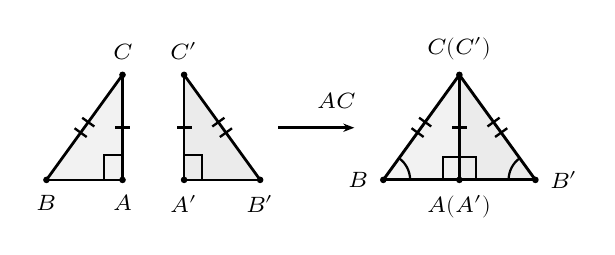
\begin{tikzpicture}[scale=0.92, every node/.style={font=\footnotesize, text=black}]
  % △ABC
  \begin{scope}[shift={(0,0)}]
    \coordinate (B) at (-1.05,0);
    \coordinate (A) at (0,0);
    \coordinate (C) at (0,1.45);
    \fill[gray!10] (B) -- (C) -- (A) -- cycle;
    \draw[black, line width=1.0pt] (B) -- (A);
    \draw[black, line width=1.0pt, tk1] (A) -- (C);
    \draw[black, line width=1.0pt, tk2] (B) -- (C);
    \rightbox[0.24]{C}{A}{B}
    \fill[black] (A) circle (1.3pt) node[below=2pt] {$A$};
    \fill[black] (B) circle (1.3pt) node[below=2pt] {$B$};
    \fill[black] (C) circle (1.3pt) node[above=2pt] {$C$};
  \end{scope}
  % △A'B'C'
  \begin{scope}[shift={(0.85,0)}]
    \coordinate (Ap) at (0,0);
    \coordinate (Bp) at (1.05,0);
    \coordinate (Cp) at (0,1.45);
    \fill[gray!16] (Ap) -- (Cp) -- (Bp) -- cycle;
    \draw[black, line width=1.0pt] (Ap) -- (Bp);
    \draw[black, line width=1.0pt, tk1] (Ap) -- (Cp);
    \draw[black, line width=1.0pt, tk2] (Bp) -- (Cp);
    \rightbox[0.24]{Cp}{Ap}{Bp}
    \fill[black] (Ap) circle (1.3pt) node[below=2pt] {$A'$};
    \fill[black] (Bp) circle (1.3pt) node[below=2pt] {$B'$};
    \fill[black] (Cp) circle (1.3pt) node[above=2pt] {$C'$};
  \end{scope}
  \draw[black, line width=0.95pt, -{Stealth[length=4pt]}] (2.15,0.72) -- (3.20,0.72) node[midway, above=3pt] {ផ្គុំ $AC$};
  % រូបផ្គុំ △BCB'
  \begin{scope}[shift={(4.65,0)}]
    \coordinate (A) at (0,0);
    \coordinate (C) at (0,1.45);
    \coordinate (B) at (-1.05,0);
    \coordinate (Bp) at (1.05,0);
    \fill[gray!10] (B) -- (C) -- (A) -- cycle;
    \fill[gray!16] (A) -- (C) -- (Bp) -- cycle;
    \draw[black, line width=1.05pt] (B) -- (Bp);
    \draw[black, line width=1.05pt, tk1] (A) -- (C);
    \draw[black, line width=1.05pt, tk2] (C) -- (B);
    \draw[black, line width=1.05pt, tk2] (C) -- (Bp);
    \rightbox[0.22]{C}{A}{B}
    \rightbox[0.22]{C}{A}{Bp}
    \draw[black, line width=0.8pt] (-0.68,0) arc (0:54:0.37);
    \draw[black, line width=0.8pt] (0.68,0) arc (180:126:0.37);
    \fill[black] (A) circle (1.3pt) node[below=2pt] {$A(A')$};
    \fill[black] (C) circle (1.3pt) node[above=2pt] {$C(C')$};
    \fill[black] (B) circle (1.3pt) node[left=2pt] {$B$};
    \fill[black] (Bp) circle (1.3pt) node[right=2pt] {$B'$};
  \end{scope}
\end{tikzpicture}}

% ៧. E3 Explain: ទ្រឹស្ដីបទប្រសព្វពុះមុំក្នុង (ទំព័រ ១៥៦)
\newcommand{\figIncenterThm}{%
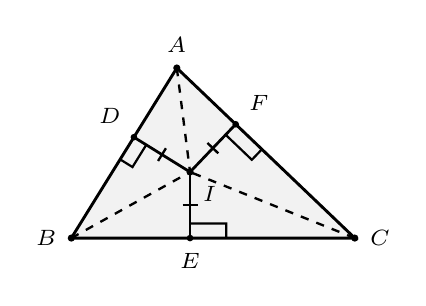
\begin{tikzpicture}[scale=1.00, every node/.style={font=\footnotesize, text=black}]
  \coordinate (B) at (0,0);
  \coordinate (C) at (3.60,0);
  \coordinate (A) at (1.34,2.16);
  \coordinate (I) at (1.508,0.839);
  \coordinate (D) at ($(B)!(I)!(A)$);
  \coordinate (E) at ($(B)!(I)!(C)$);
  \coordinate (F) at ($(A)!(I)!(C)$);
  \fill[gray!10] (A) -- (B) -- (C) -- cycle;
  \draw[black, line width=1.05pt] (A) -- (B) -- (C) -- cycle;
  \draw[black, line width=0.85pt, dashed] (A) -- (I) (B) -- (I) (C) -- (I);
  \draw[black, line width=1.0pt, tk1] (I) -- (D);
  \draw[black, line width=1.0pt, tk1] (I) -- (E);
  \draw[black, line width=1.0pt, tk1] (I) -- (F);
  \rightbox[0.22]{I}{D}{B}
  \rightbox[0.22]{I}{E}{C}
  \rightbox[0.22]{I}{F}{C}
  \fill[black] (A) circle (1.3pt) node[above=2pt] {$A$};
  \fill[black] (B) circle (1.3pt) node[left=2pt] {$B$};
  \fill[black] (C) circle (1.3pt) node[right=2pt] {$C$};
  \fill[black] (I) circle (1.3pt) node[below right=1.5pt] {$I$};
  \fill[black] (D) circle (1.2pt) node[above left=1.5pt] {$D$};
  \fill[black] (E) circle (1.2pt) node[below=2pt] {$E$};
  \fill[black] (F) circle (1.2pt) node[above right=1.5pt] {$F$};
\end{tikzpicture}}

% ៨. E4 Elaborate: លំហាត់គំរូ (ទំព័រ ១៥៥) — SCALENE △ABC, DASHED AI, ហាមគូស / លើ AD,BD,BE,AF និងធ្នូ ∠A!
\newcommand{\figModelHL}{%
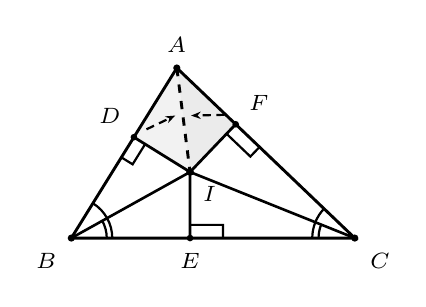
\begin{tikzpicture}[scale=1.00, every node/.style={font=\footnotesize, text=black}]
  \coordinate (B) at (0,0);
  \coordinate (C) at (3.60,0);
  \coordinate (A) at (1.34,2.16);
  \coordinate (I) at (1.508,0.839);
  \coordinate (D) at ($(B)!(I)!(A)$);
  \coordinate (E) at ($(B)!(I)!(C)$);
  \coordinate (F) at ($(A)!(I)!(C)$);
  \fill[gray!10] (A) -- (D) -- (I) -- cycle;
  \fill[gray!16] (A) -- (F) -- (I) -- cycle;
  \draw[black, line width=1.05pt] (A) -- (B) -- (C) -- cycle;
  \draw[black, line width=0.95pt] (B) -- (I) (C) -- (I);
  \draw[black, line width=1.05pt, dashed] (A) -- (I);
  \draw[black, line width=1.0pt] (I) -- (D) (I) -- (E) (I) -- (F);
  \rightbox[0.20]{I}{D}{B}
  \rightbox[0.20]{I}{E}{C}
  \rightbox[0.20]{I}{F}{C}
  % ធ្នូពុះមុំត្រង់ B និង C តែប៉ុណ្ណោះ (ហាមគូសធ្នូត្រង់ A!)
  \draw[black, line width=0.8pt] (0.45,0) arc (0:29:0.45);
  \draw[black, line width=0.8pt] (0.52,0) arc (0:58:0.52);
  \draw[black, line width=0.8pt] (3.14,0) arc (180:158:0.46);
  \draw[black, line width=0.8pt] (3.06,0) arc (180:136:0.54);
  % ព្រួញ [tracing] ពីប្រអប់កែង D, F ទៅអ៊ីប៉ូតេនុសរួម AI
  \draw[hypArrow] ($(D)+(0.16,0.10)$) -- ($(A)!0.48!(I)+(-0.10,0.03)$);
  \draw[hypArrow] ($(F)+(-0.14,0.12)$) -- ($(A)!0.48!(I)+(0.10,0.03)$);
  \fill[black] (A) circle (1.3pt) node[above=2pt] {$A$};
  \fill[black] (B) circle (1.3pt) node[below left=2pt] {$B$};
  \fill[black] (C) circle (1.3pt) node[below right=2pt] {$C$};
  \fill[black] (I) circle (1.4pt) node[below right=1.5pt] {$I$};
  \fill[black] (D) circle (1.2pt) node[above left=1.5pt] {$D$};
  \fill[black] (E) circle (1.2pt) node[below=2pt] {$E$};
  \fill[black] (F) circle (1.2pt) node[above right=1.5pt] {$F$};
\end{tikzpicture}}

% ៩. E5 Evaluate: ប្រតិបត្តិ (ទំព័រ ១៥៦) — រូបគោល △ABC (លើ) + រូបបំបែក △MDB & △MEC (ក្រោម)
\newcommand{\figPracticeHL}{%
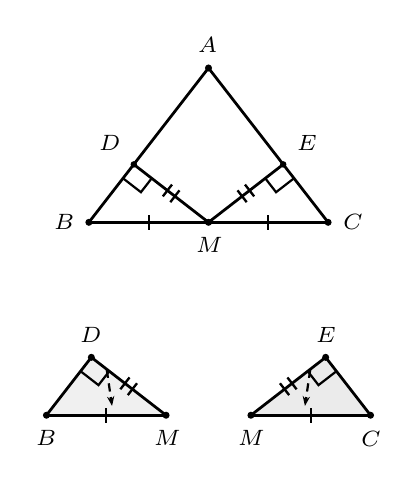
\begin{tikzpicture}[scale=0.98, every node/.style={font=\footnotesize, text=black}]
  % រូបគោល (M ចំណុចកណ្ដាល BC, MD⊥AB, ME⊥AC, MD=ME)
  \begin{scope}[shift={(0, 2.50)}]
    \coordinate (B) at (0,0);
    \coordinate (C) at (3.10,0);
    \coordinate (A) at (1.55,2.00);
    \coordinate (M) at (1.55,0);
    \coordinate (D) at ($(A)!(M)!(B)$);
    \coordinate (E) at ($(A)!(M)!(C)$);
    \draw[black, line width=1.0pt] (B) -- (A) -- (C);
    \draw[black, line width=1.0pt, tk1] (B) -- (M);
    \draw[black, line width=1.0pt, tk1] (M) -- (C);
    \draw[black, line width=1.0pt, tk2] (M) -- (D);
    \draw[black, line width=1.0pt, tk2] (M) -- (E);
    \rightbox[0.24]{M}{D}{B}
    \rightbox[0.24]{M}{E}{C}
    \fill[black] (A) circle (1.3pt) node[above=2pt] {$A$};
    \fill[black] (B) circle (1.3pt) node[left=2pt] {$B$};
    \fill[black] (C) circle (1.3pt) node[right=2pt] {$C$};
    \fill[black] (M) circle (1.3pt) node[below=2pt] {$M$};
    \fill[black] (D) circle (1.2pt) node[above left=1.5pt] {$D$};
    \fill[black] (E) circle (1.2pt) node[above right=1.5pt] {$E$};
  \end{scope}
  % បំបែក △MDB (ក្រោមឆ្វេង)
  \begin{scope}[shift={(-0.55,0)}]
    \coordinate (B1) at (0,0);
    \coordinate (M1) at (1.55,0);
    \coordinate (A1) at (1.55,2.00);
    \coordinate (D1) at ($(A1)!(M1)!(B1)$);
    \fill[gray!12] (B1) -- (D1) -- (M1) -- cycle;
    \draw[black, line width=1.0pt] (B1) -- (D1);
    \draw[black, line width=1.0pt, tk2] (D1) -- (M1);
    \draw[black, line width=1.05pt, tk1] (B1) -- (M1);
    \rightbox[0.24]{M1}{D1}{B1}
    \draw[hypArrow] ($(D1)+(0.20,-0.16)$) -- (0.85,0.12);
    \fill[black] (B1) circle (1.3pt) node[below=2pt] {$B$};
    \fill[black] (M1) circle (1.3pt) node[below=2pt] {$M$};
    \fill[black] (D1) circle (1.3pt) node[above=2pt] {$D$};
  \end{scope}
  % បំបែក △MEC (ក្រោមស្ដាំ)
  \begin{scope}[shift={(2.10,0)}]
    \coordinate (M2) at (0,0);
    \coordinate (C2) at (1.55,0);
    \coordinate (A2) at (0,2.00);
    \coordinate (E2) at ($(A2)!(M2)!(C2)$);
    \fill[gray!16] (M2) -- (E2) -- (C2) -- cycle;
    \draw[black, line width=1.0pt] (C2) -- (E2);
    \draw[black, line width=1.0pt, tk2] (M2) -- (E2);
    \draw[black, line width=1.05pt, tk1] (M2) -- (C2);
    \rightbox[0.24]{M2}{E2}{C2}
    \draw[hypArrow] ($(E2)+(-0.20,-0.16)$) -- (0.70,0.12);
    \fill[black] (M2) circle (1.3pt) node[below=2pt] {$M$};
    \fill[black] (C2) circle (1.3pt) node[below=2pt] {$C$};
    \fill[black] (E2) circle (1.3pt) node[above=2pt] {$E$};
  \end{scope}
\end{tikzpicture}}

% ១០. E5 Evaluate: រូបសង្ខេបកាតត្រួតពិនិត្យ A-B & C-D (បំបែកជា ២ ជួរច្បាស់)
\newcommand{\figExitCardsHLab}{%
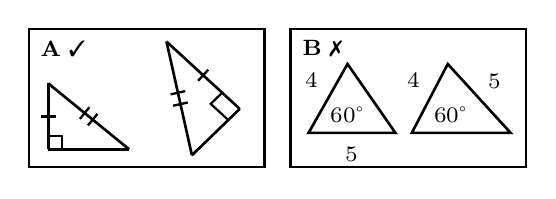
\begin{tikzpicture}[scale=0.95, every node/.style={font=\footnotesize, text=black}]
  % កាត A: អ.ជ (HL) បង្វិល ~135° ✓
  \begin{scope}[shift={(0, 0)}]
    \draw[black, line width=0.85pt] (0,0) rectangle (3.15,1.85);
    \node[anchor=north west, inner sep=3pt] at (0.04,1.81) {\textbf{A} \ding{51}};
    \draw[black, line width=0.95pt] (0.26,0.24) -- (1.34,0.24);
    \draw[black, line width=0.95pt, tk1] (0.26,0.24) -- (0.26,1.12);
    \draw[black, line width=0.95pt, tk2] (0.26,1.12) -- (1.34,0.24);
    \draw[black, line width=0.8pt] (0.26,0.42) -- (0.44,0.42) -- (0.44,0.24);
    \coordinate (Ap) at (2.82,0.78);
    \coordinate (Bp) at (2.18,0.16);
    \coordinate (Cp) at (1.84,1.68);
    \draw[black, line width=0.95pt] (Ap) -- (Bp);
    \draw[black, line width=0.95pt, tk1] (Ap) -- (Cp);
    \draw[black, line width=0.95pt, tk2] (Bp) -- (Cp);
    \rightbox[0.24]{Bp}{Ap}{Cp}
  \end{scope}
  % កាត B: អន្ទាក់ 60° SAS-vs-SSA (4cm, 5cm) ✗
  \begin{scope}[shift={(3.50, 0)}]
    \draw[black, line width=0.85pt] (0,0) rectangle (3.15,1.85);
    \node[anchor=north west, inner sep=3pt] at (0.04,1.81) {\textbf{B} \ding{55}};
    \draw[black, line width=0.95pt] (0.24,0.46) -- (1.40,0.46) -- (0.76,1.38) -- cycle;
    \node at (0.76,0.70) {$60^\circ$};
    \node[above left=0pt] at (0.50,0.94) {$4$};
    \node[below=1pt] at (0.82,0.44) {$5$};
    \draw[black, line width=0.95pt] (1.62,0.46) -- (2.94,0.46) -- (2.10,1.38) -- cycle;
    \node at (2.14,0.70) {$60^\circ$};
    \node[above left=0pt] at (1.86,0.94) {$4$};
    \node[above right=0pt] at (2.52,0.92) {$5$};
  \end{scope}
\end{tikzpicture}}
\newcommand{\figExitCardsHLcd}{%
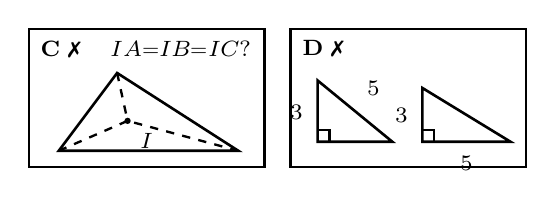
\begin{tikzpicture}[scale=0.95, every node/.style={font=\footnotesize, text=black}]
  % កាត C: IA=IB=IC? (ខុស!) ✗
  \begin{scope}[shift={(0, 0)}]
    \draw[black, line width=0.85pt] (0,0) rectangle (3.15,1.85);
    \node[anchor=north west, inner sep=3pt] at (0.04,1.81) {\textbf{C} \ding{55}};
    \coordinate (Bc) at (0.40,0.22);
    \coordinate (Cc) at (2.80,0.22);
    \coordinate (Ac) at (1.18,1.26);
    \coordinate (Ic) at (1.32,0.62);
    \draw[black, line width=0.95pt] (Ac) -- (Bc) -- (Cc) -- cycle;
    \draw[black, line width=0.85pt, dashed] (Ac) -- (Ic) (Bc) -- (Ic) (Cc) -- (Ic);
    \fill[black] (Ic) circle (1.2pt) node[below right=1pt] {$I$};
    \node[anchor=north east, inner sep=3pt] at (3.10,1.81) {$IA{=}IB{=}IC?$};
  \end{scope}
  % កាត D: អ៊ីប៉ូ vs ជ្រុង 5 cm ✗
  \begin{scope}[shift={(3.50, 0)}]
    \draw[black, line width=0.85pt] (0,0) rectangle (3.15,1.85);
    \node[anchor=north west, inner sep=3pt] at (0.04,1.81) {\textbf{D} \ding{55}};
    \draw[black, line width=0.95pt] (0.36,0.34) -- (0.36,1.16) -- (1.36,0.34) -- cycle;
    \draw[black, line width=0.8pt] (0.36,0.50) -- (0.52,0.50) -- (0.52,0.34);
    \node[above right=1pt] at (0.86,0.78) {$5$};
    \node[left=1pt] at (0.34,0.74) {$3$};
    \draw[black, line width=0.95pt] (1.76,0.34) -- (1.76,1.06) -- (2.94,0.34) -- cycle;
    \draw[black, line width=0.8pt] (1.76,0.50) -- (1.92,0.50) -- (1.92,0.34);
    \node[below=1pt] at (2.35,0.32) {$5$};
    \node[left=1pt] at (1.74,0.70) {$3$};
  \end{scope}
\end{tikzpicture}}

% ១១ក. ជំហានទី៥ កិច្ចការផ្ទះ៖ លំហាត់ទី១០ (ទំ.១៦៥) + បំបែក ΔBDC, ΔCEB
\newcommand{\figHWtenHL}{%
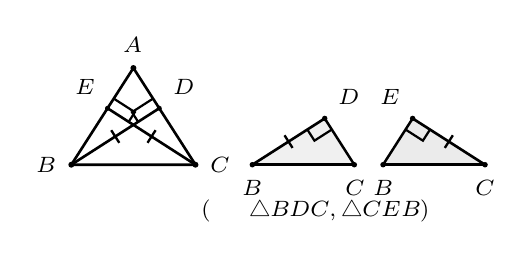
\begin{tikzpicture}[scale=0.83, every node/.style={font=\footnotesize, text=black}]
  \begin{scope}[shift={(-2.15,0)}]
    \coordinate (A) at (0,1.48);
    \coordinate (B) at (-0.95,0);
    \coordinate (C) at (0.95,0);
    \coordinate (D) at ($(A)!(B)!(C)$);
    \coordinate (E) at ($(A)!(C)!(B)$);
    \draw[black, line width=0.95pt] (A) -- (B) -- (C) -- cycle;
    \draw[black, line width=0.95pt, tk1] (B) -- (D);
    \draw[black, line width=0.95pt, tk1] (C) -- (E);
    \rightbox[0.24]{B}{D}{A}
    \rightbox[0.24]{C}{E}{A}
    \fill[black] (A) circle (1.3pt) node[above=2pt] {$A$};
    \fill[black] (B) circle (1.3pt) node[left=2pt] {$B$};
    \fill[black] (C) circle (1.3pt) node[right=2pt] {$C$};
    \fill[black] (D) circle (1.1pt) node[above right=1.5pt] {$D$};
    \fill[black] (E) circle (1.1pt) node[above left=1.5pt] {$E$};
  \end{scope}
  \begin{scope}[shift={(0.45,0)}]
    \coordinate (B1) at (-0.78,0);
    \coordinate (C1) at (0.78,0);
    \coordinate (A1) at (0,1.22);
    \coordinate (D1) at ($(A1)!(B1)!(C1)$);
    \fill[gray!12] (B1) -- (D1) -- (C1) -- cycle;
    \draw[black, line width=0.9pt] (D1) -- (C1);
    \draw[black, line width=1.05pt] (B1) -- (C1);
    \draw[black, line width=0.95pt, tk1] (B1) -- (D1);
    \rightbox[0.24]{B1}{D1}{C1}
    \fill[black] (B1) circle (1.2pt) node[below=2pt] {$B$};
    \fill[black] (C1) circle (1.2pt) node[below=2pt] {$C$};
    \fill[black] (D1) circle (1.2pt) node[above right=1.5pt] {$D$};
  \end{scope}
  \begin{scope}[shift={(2.45,0)}]
    \coordinate (B2) at (-0.78,0);
    \coordinate (C2) at (0.78,0);
    \coordinate (A2) at (0,1.22);
    \coordinate (E2) at ($(A2)!(C2)!(B2)$);
    \fill[gray!16] (B2) -- (E2) -- (C2) -- cycle;
    \draw[black, line width=0.9pt] (B2) -- (E2);
    \draw[black, line width=1.05pt] (B2) -- (C2);
    \draw[black, line width=0.95pt, tk1] (C2) -- (E2);
    \rightbox[0.24]{C2}{E2}{B2}
    \fill[black] (B2) circle (1.2pt) node[below=2pt] {$B$};
    \fill[black] (C2) circle (1.2pt) node[below=2pt] {$C$};
    \fill[black] (E2) circle (1.2pt) node[above left=1.5pt] {$E$};
  \end{scope}
  \node[below=6pt] at (0.10,-0.14) {លំហាត់ទី១០ (បំបែក $\tri{BDC}, \tri{CEB}$)};
\end{tikzpicture}}

% ១១ខ. ជំហានទី៥ កិច្ចការផ្ទះ៖ លំហាត់ទី១២ (ទំ.១៦៥)
\newcommand{\figHWtwelveHL}{%
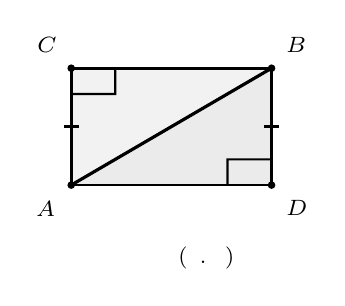
\begin{tikzpicture}[scale=1.06, every node/.style={font=\footnotesize, text=black}]
  \coordinate (A) at (0,0);
  \coordinate (D) at (2.40,0);
  \coordinate (C) at (0,1.40);
  \coordinate (B) at (2.40,1.40);
  \fill[gray!10] (A) -- (C) -- (B) -- cycle;
  \fill[gray!16] (A) -- (B) -- (D) -- cycle;
  \draw[black, line width=0.95pt] (C) -- (B) (A) -- (D);
  \draw[black, line width=0.95pt, tk1] (A) -- (C);
  \draw[black, line width=0.95pt, tk1] (B) -- (D);
  \draw[black, line width=1.15pt] (A) -- (B);
  \rightbox[0.22]{A}{C}{B}
  \rightbox[0.22]{B}{D}{A}
  \fill[black] (A) circle (1.3pt) node[below left=2pt] {$A$};
  \fill[black] (B) circle (1.3pt) node[above right=2pt] {$B$};
  \fill[black] (C) circle (1.3pt) node[above left=2pt] {$C$};
  \fill[black] (D) circle (1.3pt) node[below right=2pt] {$D$};
  \node[below=14pt] at (1.20,-0.16) {លំហាត់ទី១២ (ទំ.១៦៥)};
\end{tikzpicture}}

% ============================================================================
% ចាប់ផ្ដើមឯកសារ (Document Body)
% ============================================================================
\begin{document}
\fontsize{10pt}{15.2pt}\selectfont

% -------------------- ក្បាលកិច្ចតែងការ (Header) --------------------
\begin{center}
  {\muol\fontsize{11pt}{16pt}\selectfont ព្រះរាជាណាចក្រកម្ពុជា}\\[2pt]
  {\muol\fontsize{10pt}{15pt}\selectfont ជាតិ សាសនា ព្រះមហាក្សត្រ}\\[1pt]
  \khmflourish
\end{center}

\vspace{-11pt}
{\muol\fontsize{9.5pt}{13.2pt}\selectfont
មន្ទីរអប់រំ យុវជន និងកីឡា ខេត្តកំពង់ធំ\\
ការិយាល័យអប់រំ យុវជន និងកីឡា ស្រុកកំពង់ស្វាយ\\
អនុវិទ្យាល័យព្រះក្រសាំង}

\vspace{2pt}
\begin{center}
  {\muol\fontsize{10pt}{15pt}\selectfont កិច្ចតែងការបង្រៀន}
\end{center}
\vspace{1pt}

% -------------------- ព័ត៌មានទូទៅ (Metadata) --------------------
{\renewcommand{\arraystretch}{1.06}
\hspace*{3.30cm}%
\begin{tabular}{@{}l l l@{}}
  - \hspace{0.35cm} មុខវិជ្ជា & : & គណិតវិទ្យា ថ្នាក់ទី៨ \\
  - \hspace{0.35cm} ចំណងជើងមេរៀន & : & មេរៀនទី១២ ការប្រៀបធៀបត្រីកោណ \\
  - \hspace{0.35cm} ចំណងជើងរង & : & ១.៣. លក្ខខណ្ឌចំពោះត្រីកោណកែងប៉ុនគ្នា \\
  & & ១.៣.២ អ៊ីប៉ូតេនុសប៉ុនគ្នា និងជ្រុងមុំកែងមួយប៉ុនគ្នា (អ.ជ) និងប្រសព្វពុះមុំក្នុងត្រីកោណ \\
  - \hspace{0.35cm} រយៈពេល & : & ១ ម៉ោងសិក្សា (៥០នាទី) \\
  - \hspace{0.35cm} បង្រៀនដោយ & : & ហុក ប៊ុនថែន \\
  - \hspace{0.35cm} កាលបរិច្ឆេទ & : & ថ្ងៃចន្ទ ទី៣០ ខែវិច្ឆិកា ឆ្នាំ២០២៦ \\
\end{tabular}

\vspace{2pt}

% -------------------- I. វត្ថុបំណង --------------------
\textbf{I.} {\muol វត្ថុបំណង}\\[2pt]
\hspace*{0.55cm}%
\begin{tabular}{@{}l l l@{}}
  \wcirc \hspace{0.25cm} វិជ្ជាសម្បទា & : & សិស្សកំណត់បានលក្ខខណ្ឌ អ.ជ (HL) តាមពិសោធន៍ត្រឡប់កែង $3$-$4$-$5\text{ cm}$ ទល់នឹងអន្ទាក់ $35^\circ$ (ជ.ជ.ម) \\
  & & រៀបរាប់សម្រាយ $90^\circ{+}90^\circ=180^\circ\to$ អ.ម (កែទំ.១៥៤) និងទ្រឹស្ដីបទប្រសព្វពុះមុំក្នុងត្រីកោណ ។ \\
  \wcirc \hspace{0.25cm} បំណិនសម្បទា & : & សិស្សបត់ក្រដាស $\tri{ABC}$ រកផ្ចិត $I$, ប្រើ \textbf{[tracing]} ខ្សែសង្វាក់ អ.ម $\to$ អ.ជ, ធនាគារហេតុផល \cnum{1}--\cnum{5} \\
  & & និងបំបែក $\tri{MDB}, \tri{MEC}$ ដើម្បីស្រាយបញ្ជាក់ ព្រមទាំងញែក $ID=IE=IF$ ពី $IA, IB, IC$ ។ \\
  \wcirc \hspace{0.25cm} ចរិយាសម្បទា & : & សិស្សសហការជា «ក្រុមវិស្វករសួនរង្វង់ត្រីកោណ» ហ៊ានទស្សន៍ទាយដោយភស្តុតាង និងមិនបន្ថែម \\
  & & សញ្ញាស្មើ \textbf{/} មុនស្រាយ ឬច្រឡំសន្និដ្ឋានមកធ្វើជាហេតុផល ប្រកបដោយការប្រុងប្រយ័ត្ន ។ \\
\end{tabular}

\vspace{2pt}

% -------------------- II. សម្ភារៈឧបទេស --------------------
\textbf{II.} {\muol សម្ភារៈឧបទេស}\\[2pt]
\hspace*{0.55cm}$\bullet$ \hspace{0.35cm} សៀវភៅគោលទី៨ (ទំ.១៥៤--១៥៦, ១៦៥) កន្ត្រៃ បន្ទាត់ រ៉ាព័រទ័រ ដែកឈាន កញ្ចប់ ១:១ (ទំព័រ ១) កាត E4--E5 ផ្ទាំង \cnum{1}--\cnum{5} កាត A--D (ស-ខ្មៅ)

\vspace{2pt}

% -------------------- III. វិធីសាស្រ្តបង្រៀន --------------------
\textbf{III.} {\muol វិធីសាស្រ្តបង្រៀន}\\[2pt]
\hspace*{0.55cm}%
\begin{tabular}{@{}l l l@{}}
  $\bullet$ \hspace{0.35cm} គោលវិធី & : \hspace{0.7cm} & សិស្សមជ្ឈមណ្ឌល \\
  $\bullet$ \hspace{0.35cm} យុទ្ធវិធីបង្រៀន & : & ស្ថាបនានិយម គម្រូ 5Es (ត្រឡប់ $90^\circ$ បត់ POE ផែនទី \textbf{[tracing]} \& តុសវនកម្ម ៣ តួនាទី) \\
\end{tabular}
}

\vspace{2pt}

% -------------------- IV. ដំណើរការបង្រៀន --------------------
\textbf{IV.} {\muol ដំណើរការបង្រៀន}

% ============================================================================
% តារាងដំណើរការបង្រៀន (Modular Multi-Row 3-Column Table – 50 នាទី)
% ============================================================================
\renewcommand{\arraystretch}{1.15}
\begin{longtable}{|L{5.50cm}|L{7.90cm}|L{4.80cm}|}
\hline
\rowcolor{headgray}
\multicolumn{1}{|c|}{\muol សកម្មភាពគ្រូ} &
\multicolumn{1}{c|}{\muol ខ្លឹមសារមេរៀន} &
\multicolumn{1}{c|}{\muol សកម្មភាពសិស្ស} \\
\hline
\endfirsthead

\hline
\endhead

\hline
\endfoot

\hline
\endlastfoot

% ==================== ជំហានទី១ (2min) ====================
\stepheader{ជំហានទី១ \enbf{(}រដ្ឋបាលថ្នាក់\enbf{)}}
- ពិនិត្យអវត្តមាន និងអនាម័យថ្នាក់រៀន \newline
- ចាត់ក្រុម ៣ នាក់ («ក្រុមវិស្វករសួនរង្វង់ត្រីកោណ») \newline
- ចែកសន្លឹកកិច្ចការទំព័រ ១ (១:១) ទុកលើតុ
&
\hspace*{0.3cm}- រដ្ឋបាលថ្នាក់ \newline
\hspace*{0.3cm}- អនាម័យ និងសណ្ដាប់ធ្នាប់ថ្នាក់រៀន \newline
\hspace*{0.3cm}- ត្រៀមក្រុមវិស្វករសួនរង្វង់ត្រីកោណ
&
- រាយការណ៍អវត្តមាន \newline
- អង្គុយតាមក្រុម ៣ នាក់ \newline
- ទទួលសន្លឹកកិច្ចការទុកលើតុ \\
\hline

% ==================== ជំហានទី២ (9min: HW <=3m + Prereq <=3m + E1 3m) ====================
\stepheader{ជំហានទី២ \enbf{(}កិច្ចការផ្ទះ \enbf{+} ទំនាក់ទំនងមេរៀនថ្មី\enbf{)}}
% --- ២.១ កំណែកិច្ចការផ្ទះ៖ អន្ទាក់លំហាត់ទី៦ ---
- ពិនិត្យកិច្ចការផ្ទះ (លំហាត់ទី៦ និងទី៧) \newline
\ditem \textbf{សំណួរបញ្ឆោត} ៖ «ក្នុងលំហាត់ទី៦ តើ $AD$ ជាអ៊ីប៉ូតេនុស ឬជាជ្រុងមុំកែង?» \newline
\timenote{ចំណាយពេលឱ្យតិចបំផុតកុំឱ្យលើស 3min}
&
\centerline{\redsub{កំណែកិច្ចការផ្ទះ (លំហាត់ \#6 ទំ.១៦៤ \& \#7 ទំ.១៦៥)}}
\centerline{\underline{ចម្លើយសង្ខេប}}
- ទី៦៖ $AD$ ជាជ្រុងកែងរួម $\Rightarrow \tri{ABD}\cg\tri{ACD}$ (ម.ជ.ម) $\Rightarrow AB=AC$ \newline
- ទី៧៖ ក. $PB=PC$ (ជ.ម.ជ) $\vert$ ខ. $PH=PK$ \graybox{(លក្ខខណ្ឌ អ.ម)}
&
- ផ្ទៀង និងឆ្លើយ៖ \newline
«$AD$ ជាជ្រុងមុំកែងរួម មិនមែនអ៊ីប៉ូតេនុសទេ ដូច្នេះប្រើ ម.ជ.ម!» \\[3pt]

&
\cfig{\figHWoldHL}
& \\[3pt]

% --- ២.២ រំលឹកមេរៀនទាក់ទង (<=3min) ---
\ditem \textbf{រំលឹករហ័ស (ភាគ ១--២)} ៖ \newline
+ បើ $\ang{BAC}+\ang{CAB'}=90^\circ{+}90^\circ$ តើ $B, A, B'$ ដូចម្ដេច? បើ $CB=CB'$ តើ $\ang{B}$ និង $\ang{B'}$ ស្មើគ្នាឬ? \newline
+ តើករណី អ.ម និងលក្ខណៈផ្ទាល់ពុះមុំនិយាយដូចម្ដេច? \newline
\timenote{រួមទាំងពីរកុំឱ្យលើស 3min}
&
\centerline{\redsub{រំលឹកមេរៀនទាក់ទងមេរៀនថ្មី}}
- មុំរាប $\ang{BAB'}=180^\circ \Rightarrow B, A, B'$ ត្រង់ជួរ ($BB'$) \newline
- ត្រីកោណសមបាទ $CB=CB'\Rightarrow \ang{B}=\ang{B'}$ \newline
- អ.ម (HA)៖ អ៊ីប៉ូតេនុស + មុំស្រួច \newline
- ពុះមុំផ្ទាល់៖ $MA=MB$
&
- ឆ្លើយ៖ \newline
«$B, A, B'$ ត្រង់ជួរ $\ang{B}=\ang{B'}$ និងចំណុចលើពុះមុំស្មើចម្ងាយពីជ្រុងទាំងពីរ» \\[3pt]

&
\cfig{\figPrereqHL}
& \\[3pt]

% --- ២.៣ E1 Engage: អាងទឹករង្វង់សួនផ្លូវប្រសព្វ ៣ ខ្សែ ---
\fiveE{E1 - Engage (3min)} \newline
\ditem \textbf{អាងទឹករង្វង់សួនផ្លូវប្រសព្វ ៣ ខ្សែ និងអាថ៌កំបាំងរួចផុតពីអន្ទាក់ ជ.ជ.ម} ៖ \newline
+ វិស្វករទាញពុះមុំ $\ang{B}, \ang{C}$ ប្រសព្វត្រង់ $I$ \newline
+ រួចក្រាលផ្លូវកែង $ID, IE, IF$ ទៅជ្រុងទាំងបី
&
\centerline{\redsub{ស្ថានភាពពិត៖ អាងទឹករង្វង់សួនប្រសព្វ ៣ ផ្លូវ}}
\textbf{ចម្ងល់ ១៖} ហេតុអ្វី $ID=IE=IF$? \newline
\textbf{ចម្ងល់ ២៖} ហេតុអ្វី $AI$ ពុះ $\ang{A}$ ទាំងមានតែ $90^\circ$ (មិននៅចន្លោះ)?
&
- ពិនិត្យស្ថានភាពពិតអាងទឹកសួន \newline
- ទស្សន៍ទាយមូលហេតុ $ID=IE=IF$ \newline
- ទស្សន៍ទាយ $AI$ ពុះ $\ang{A}$ ផុតអន្ទាក់ ជ.ជ.ម \\[3pt]

&
\cfig{\figEngageHL}
& \\
\hline

% ==================== ជំហានទី៣ (17min: E2 11m + E3 6m) ====================
\stepheader{ជំហានទី៣ \enbf{(}ខ្លឹមសារមេរៀនថ្មី\enbf{)}}
% --- ៣.១ ចំណងជើង & E2 Act 1 (6min) ---
- សរសេរចំណងជើងមេរៀនលើក្ដារខៀន \newline
\fiveE{E2 - Explore (11min)} \newline
\ditem \textbf{សកម្មភាព ១៖ ត្រឡប់ខ្នង $3$-$4$-$5\text{cm}$ vs ធ្នូ $35^\circ$ (6min)} \newline
+ កាត់ $\tri{ABC}, \tri{A'B'C'}$ លើទំព័រ ១ ($AC=A'C'=3\text{cm}, BC=B'C'=5\text{cm}$) ត្រឡប់ផ្គុំ $A'C'$ លើ $AC$ \newline
+ ធៀបនឹងធ្នូ ជ.ជ.ម $35^\circ$ ($PQ=4\text{cm}, r=2.8\text{cm}$)
&
មេរៀនទី១២ \hspace{0.1cm} {\muol ការប្រៀបធៀបត្រីកោណ} \textbf{(ត)} \newline
១.៣. លក្ខខណ្ឌចំពោះត្រីកោណកែងប៉ុនគ្នា \newline
១.៣.២ អ៊ីប៉ូតេនុសប៉ុនគ្នា និងជ្រុងមុំកែងមួយប៉ុនគ្នា (អ.ជ) និងប្រសព្វពុះមុំក្នុងត្រីកោណ \newline
+ $90^\circ$ បង្ខំ $\ang{BAB'}=180^\circ$ ($\tri{BCB'}$ សមបាទ) ប៉ុន្តែ $35^\circ$ កាត់ $2$ កន្លែង!
&
- កត់ចំណងជើង \newline
- ផ្គុំ $A'C'=AC$ ឃើញត្រួត ១០០\% \newline
- សង្កេតធ្នូកាត់ $R_1, R_2$ \\[3pt]

&
\cfig{\figExploreOneHL}
& \\[3pt]

% --- ៣.២ E2 Act 2 (5min POE): បត់ក្រដាស scalene △ABC រកផ្ចិត I ---
\ditem \textbf{សកម្មភាព ២៖ POE បត់ពុះមុំ $\tri{ABC}$ សាមញ្ញ (5min)} \newline
+ \textbf{P}៖ ទាយថាផ្នត់ពុះ $\ang{A}$ កាត់ $I$ ទេ? តើ $ID=IE=IF$ ឬ $IA=IB=IC$? \newline
+ \textbf{O--E}៖ បត់ពុះ $\ang{B}, \ang{C}$ រក $I$, បត់តេស្ត $\ang{A}$, រួចវាស់ $ID, IE, IF$ ធៀប $IA, IB, IC$
&
\centerline{\textbf{POE៖ បត់ពុះមុំ $\tri{ABC}$ សាមញ្ញ និងតេស្តរង្វង់ចារឹកក្នុង}}
+ $BC=9.2\text{ cm},\, AB=6.5\text{ cm},\, AC=8.0\text{ cm}$ \newline
+ \graybox{$r = ID=IE=IF\approx 2.1\text{cm}$ (រង្វង់ចារឹកក្នុង)} \newline
+ $IA\approx 3.4,\, IB\approx 4.4,\, IC\approx 5.8\text{ cm} \Rightarrow$ \graybox{$IA\neq IB\neq IC$}
&
- បត់រក $I$ និងផ្ទៀងផ្នត់ $AI$ ពុះ $\ang{A}$ \newline
- វាស់ $r\approx 2.1\text{cm}$ ធៀប $IA, IB, IC$ \\[3pt]

&
\cfig{\figExploreTwoHL}
& \\[3pt]

% --- ៣.៣ E3 Explain: សម្រាយត្រឡប់ អ.ជ (HL) កែកំហុសទំ.១៥៤ ---
\fiveE{E3 - Explain (6min)} \newline
\ditem ដឹកនាំសម្រាយត្រឡប់ $AC=A'C'$ និង\textbf{កែកំហុសទាំង ៣ ចំណុចទំព័រ ១៥៤}៖ \newline
(១) ប្រើ $AC=A'C'$ ស៊ីគ្នាទាំងអត្ថបទ-រូប (ជំនួស $AB=A'B'$) \newline
(២) កែ \textit{«(តាមលកខណ្ឌ អ.ជ)»} $\to$ \textbf{«(តាមលក្ខខណ្ឌ អ.ម)»} (លុបរង្វង់តក្ក) \newline
(៣) កែ \textit{«លកខណ្ឌ»} $\to$ \textbf{«លក្ខខណ្ឌ»}
&
\centerline{\textbf{សម្រាយទ្រឹស្ដីបទ អ.ជ (HL) — កែកំហុសសៀវភៅទំ.១៥៤}}
ក្នុង $\tri{ABC}, \tri{A'B'C'}$ ($\ang{A}=\ang{A'}=90^\circ, AC=A'C', BC=B'C'$) ត្រឡប់ផ្គុំ $A'C'$ លើ $AC$៖ \newline
+ $\ang{BAB'}=90^\circ{+}90^\circ=180^\circ \Rightarrow BB'$ អង្កត់ត្រង់ \newline
+ $\tri{BCB'}$ មាន $CB=CB'$ (សមបាទ) $\Rightarrow \ang{B}=\ang{B'}$ \newline
+ ក្នុង $\tri{BAC}, \tri{B'AC}$៖ $CB=CB', \ang{B}=\ang{B'}$ \newline
$\Rightarrow \tri{ABC}\cg\tri{A'B'C'}$ \graybox{\textbf{(តាមលក្ខខណ្ឌ អ.ម)}} ។
&
- រកឃើញកំហុសប្ដូរជ្រុង និងរង្វង់តក្កទំ.១៥៤ \newline
- យល់ថា អ.ជ ស្រាយដោយ អ.ម! \\[3pt]

&
\cfig{\figProofHL}
& \\[3pt]

% --- ៣.៤ E3 Explain: ទ្រឹស្ដីបទ អ.ជ, ប្រសព្វពុះមុំ, រូប P4, តារាង H-C-C & ធនាគារ ①–⑤ ---
\cnum{1} បង្គុំពំនោលទ្រឹស្ដីបទ \textbf{អ.ជ (HL)} (ទំ.១៥៥) និង \textbf{ប្រសព្វពុះមុំក្នុង} (ទំ.១៥៦)
&
\textbf{ទ្រឹស្ដីបទ អ.ជ (ទំ.១៥៥)៖} \newline
ត្រីកោណកែងពីរប៉ុនគ្នា កាលណាវាមានអ៊ីប៉ូតេនុសប៉ុនគ្នា និងជ្រុងនៃមុំកែងមួយប៉ុនគ្នា ។ \newline
\textbf{ទ្រឹស្ដីបទប្រសព្វពុះមុំ (ទំ.១៥៦)៖} \newline
កន្លះបន្ទាត់ពុះមុំក្នុងទាំងបីនៃត្រីកោណមួយប្រសព្វគ្នាត្រង់ចំណុចតែមួយ ($I$) ដែលឋិតនៅស្មើចម្ងាយពីជ្រុងទាំងបី ($ID=IE=IF$) ។
&
- កត់ត្រាពំនោលទ្រឹស្ដីបទទាំង ២ \\[3pt]

&
\cfig{\figIncenterThm}
& \\[3pt]

\cnum{2} បិទផ្ទាំង \textbf{ធនាគារហេតុផល អ.ជ \cnum{1}--\cnum{5}} (ទំព័រ ៤) \newline
– ផ្ទៀងតារាងសម្មតិកម្ម--សន្និដ្ឋាន--វិបាក (H--C--C)
&
\cfig{%
\small
\renewcommand{\arraystretch}{1.15}
\begin{tabular}{|c|c|c|}
  \hline
  \cellcolor{headgray} សម្មតិកម្ម (អ.ជ / HL) & \cellcolor{headgray} សន្និដ្ឋាន & \cellcolor{headgray} វិបាក (\cnum{5}) \\
  \hline
  $\ang{A}=\ang{A'}=90^\circ$ & $\tri{ABC}\cg$ & ជ្រុងសល់ស្មើ \\
  អ៊ីប៉ូ $BC=B'C'$ & $\tri{A'B'C'}$ & មុំស្រួចស្មើ \\
  ជ្រុងកែង $AC=A'C'$ & (អ.ជ / HL) & ច្រាសពុះមុំ \\[2pt]
  \hline
\end{tabular}%
}
&
- កត់ត្រាតារាង H--C--C \\[3pt]

– បញ្ជាក់ធនាគារហេតុផល \cnum{1}--\cnum{5}
&
\textbf{ធនាគារហេតុផល អ.ជ \cnum{1}--\cnum{5}៖} \newline
\cnum{1} មុំកែង $90^\circ$ $\vert$ \cnum{2} អ៊ីប៉ូតេនុសស្មើ ឬរួម (ឈម $90^\circ$)
&
- កត់ត្រាធនាគារ \cnum{1}--\cnum{5} \\[3pt]

– បញ្ជាក់ភាពខុសគ្នារវាងផ្ចិត $I, O, G$
&
\cnum{3} ជ្រុងមុំកែងស្មើ ឬរួម (ជាប់ $90^\circ$) \newline
\cnum{4} លក្ខខណ្ឌ អ.ជ (HL) $\vert$ \cnum{5} ធាតុត្រូវគ្នា / ច្រាសពុះមុំ ($ID=IF \Rightarrow AI$ ពុះ $\ang{A}$) ។ \newline
\textbf{ប្រយ័ត្នចំណុចពិសេស ៣៖} ពុះមុំ ($I$, $ID=IE=IF$ ទៅជ្រុង) $\neq$ មេដ្យាទ័រ ($O$, ស្មើកំពូល) $\neq$ មេដ្យាន ($G$, កណ្ដាលជ្រុង) ។
&
- ញែកផ្ចិត $I, O, G$ \\
\hline

% ==================== ជំហានទី៤ (20min: E4 10m + E5 10m) ====================
\stepheader{ជំហានទី៤ \enbf{(}ពង្រីកចំណេះដឹង\enbf{)}}
% --- ៤.១ E4 Elaborate: លំហាត់គំរូ (ទំព័រ ១៥៥) — ផែនទីច្រវាក់ អ.ម → អ.ជ ផ្ចិត I ---
\fiveE{E4 - Elaborate (10min)} \newline
\ditem ចែកកាត \textbf{«ផែនទីច្រវាក់ អ.ម $\to$ អ.ជ ផ្ចិត I»} (ទំព័រ ២)៖ \newline
\cnum{1} ដាស់តឿន\textbf{មិនគូស $/$ លើ $AD, BD, BE, AF$ និងធ្នូមុំ $\ang{A}$} (កែរូបទំ.១៥៥) \newline
\cnum{2} ប្រើ \textbf{[tracing]} អូស $90^\circ\to$ អ៊ីប៉ូតេនុស $BI, CI$ (ក) រួច $AI$ (ខ)
&
{\muol លំហាត់គំរូ} \textbf{(ទំព័រ ១៥៥) ៖} \newline
កន្លះបន្ទាត់ពុះនៃ $\ang{B}$ និង $\ang{C}$ ក្នុង $\tri{ABC}$ ប្រសព្វគ្នាត្រង់ $I$ ។ \newline
តាម $I$ គូសកែងនឹង $AB, BC, AC$ ត្រង់ $D, E, F$ ។ \newline
\hspace*{0.15cm}ក. បង្ហាញថា $ID=IE=IF$ \quad ខ. បង្ហាញថា $AI$ ពុះ $\ang{BAC}$ ។
&
- អូសម្រាមដៃ \textbf{[tracing]} តាមខ្សែសង្វាក់ \newline
- មិនលួចគូស $/$ ឬធ្នូ $\ang{A}$ \\[3pt]

&
\cfig{\figModelHL}
& \\[3pt]

% --- ៤.២ ចម្លើយលំហាត់គំរូ + 30s EIA Looking-Back ---
\ditem ដឹកនាំបំពេញផែនទីច្រវាក់ \cnum{1}--\cnum{5} ដំណាក់កាល ក. ($\text{អ.ម}\times 2$)
&
\centerline{\underline{\redsub{ចម្លើយខ្សែសង្វាក់ (អ.ម $\to$ អ.ជ)}}}
\textbf{ក.} $\tri{BEI}, \tri{BDI}$៖ $\ang{E}=\ang{D}=90^\circ$, $BI$ អ៊ីប៉ូតេនុសរួម, $\ang{IBE}=\ang{IBD}$ \newline
$\Rightarrow \tri{BEI}\cg\tri{BDI}$ (អ.ម) $\Rightarrow ID=IE$ (1) \newline
ដូចគ្នា $\tri{CEI}\cg\tri{CFI}$ (អ.ម៖ $\ang{E}=\ang{F}=90^\circ$, $CI$ រួម, $\ang{ICE}=\ang{ICF}$) \newline
$\Rightarrow IE=IF$ (2) $\Rightarrow$ \graybox{$ID=IE=IF$} ។
&
- សរសេរសម្រាយផ្នែក ក. ដោយប្រើ អ.ម \\[3pt]

– ដឹកនាំបំពេញដំណាក់កាល ខ. (អ.ជ) និងសួរ \textbf{EIA 30s} ($ID=IE=IF$ vs $IA, IB, IC$)
&
\textbf{ខ.} ក្នុងត្រីកោណកែង $\tri{IDA}$ និង $\tri{IFA}$ មាន៖ \newline
+ $\ang{IDA}=\ang{IFA}=90^\circ$ (\cnum{1}) \newline
+ អ៊ីប៉ូតេនុសរួម $AI$ (\cnum{2}), $ID=IF$ ពី ក. (\cnum{3}) \newline
$\Rightarrow$ \graybox{$\tri{IDA}\cg\tri{IFA}$ (\cnum{4} អ.ជ)} $\Rightarrow \ang{IAD}=\ang{IAF}$ (\cnum{5}) \newline
$\Rightarrow$ \graybox{$AI$ ពុះ $\ang{BAC}$} ។ \newline
\timenote{EIA 30s៖ ផ្ចិតពុះមុំ $I$ ស្មើចម្ងាយពីជ្រុង ៣ ($ID=IE=IF$, រង្វង់ចារឹកក្នុង) ខុសពីមេដ្យាទ័រ ($IA=IB=IC$ ស្មើទៅកំពូល) និងមេដ្យាន! ក្នុង $\tri{ABC}$ សាមញ្ញ $IA\neq IB\neq IC$ ។}
&
- សរសេរសម្រាយផ្នែក ខ. ដោយប្រើ អ.ជ \newline
- ញែក $ID=IE=IF \neq IA, IB, IC$ \\[3pt]

% --- ៤.៣ E5 Evaluate: ប្រតិបត្តិ (ទំព័រ ១៥៦) — តុសវនកម្មចំណុចកណ្ដាល–អង្កត់កែង ៣ តួនាទី ---
\fiveE{E5 - Evaluate (10min)} \newline
\ditem {\muol លំហាត់ប្រតិបត្តិ} \textbf{(ទំព័រ ១៥៦)} \newline
+ ចែកសន្លឹក \textbf{«តុសវនកម្មចំណុចកណ្ដាល--អង្កត់កែង ៣ តួនាទី»} (ទំព័រ ៣)៖ \newline
$M$ ចំណុចកណ្ដាល $BC$, $MD\perp AB, ME\perp AC$, $MD=ME$ ។ បង្ហាញថា $\ang{B}=\ang{C}$ ។
&
\centerline{{\muol ចម្លើយលំហាត់ប្រតិបត្តិ} \textbf{(រូបគោល \& រូបបំបែក)}}
&
- បំបែក $\tri{MDB}, \tri{MEC}$ \newline
- មិនមើលភ្នែកថា $AB=AC$ ទេ \\[3pt]

&
\cfig{\figPracticeHL}
& \\[3pt]

% --- ៤.៤ E5 Evaluate: លម្អិត ៣ តួនាទី (Pause-Ask / Pause-Review) ---
\ditem ចាត់វេន ៣ តួនាទី (\textbf{៣០វិ./ម្នាក់})៖ \newline
\cnum{1} \textbf{តួនាទី ១ (Pause-Ask)}៖ ពន្យល់មុនគូស $90^\circ\to$ អ៊ីប៉ូ $MB=MC$ \newline
\cnum{2} \textbf{តួនាទី ២}៖ សរសេរ \cnum{1}--\cnum{4} ($\tri{MDB}\cg\tri{MEC}$) \newline
\cnum{3} \textbf{តួនាទី ៣ (Pause-Review)}៖ ផ្ទៀង $\ang{B}=\ang{C}$ (\cnum{5}) និង\textbf{បិទ E1}
&
+ ក្នុងត្រីកោណកែង $\tri{MDB}$ និង $\tri{MEC}$ មាន៖ \newline
\hspace*{0.25cm}$\ang{MDB} = \ang{MEC} = 90^\circ$ \hspace{0.25cm} (\cnum{1} អង្កត់កែង) \newline
\hspace*{0.25cm}អ៊ីប៉ូតេនុស $MB = MC$ \hspace{0.45cm} (\cnum{2} $M$ ចំណុចកណ្ដាល $BC$) \newline
\hspace*{0.25cm}ជ្រុងកែង $MD = ME$ \hspace{0.52cm} (\cnum{3} បម្រាប់) \newline
$\Rightarrow \tri{MDB} \cg \tri{MEC}$ \hspace{0.95cm} (\cnum{4} លក្ខខណ្ឌ អ.ជ) \newline
$\Rightarrow \ang{B} = \ang{C}$ \hspace{1.75cm} (\cnum{5} មុំត្រូវគ្នា) ។
&
- អនុវត្ត ៣ តួនាទី + Pause-Ask / Pause-Review \newline
- ប្រយ័ត្នទំ.១៥៦៖ ហាមសន្មតតាមភ្នែកថា $AB=AC$ ឬប្រើ អ.ម មុនស្រាយ $\ang{B}=\ang{C}$! \\[3pt]

% --- ៤.៥ បិទ E1 & កាតត្រួតពិនិត្យ A-D (60-90s) ---
\ditem បិទបញ្ហា E1 រួចបញ្ចាំង \textbf{កាត A--D (60--90s)} (ទំព័រ ៥)៖ \newline
+ ឱ្យសិស្សចង្អុលអ៊ីប៉ូតេនុសមុនលើក \ding{51}/\ding{55} និងម្រាម ១--៣
&
\textbf{បិទ E1}៖ \graybox{$ID=IE=IF$ (អ.ម)} $\to$ \graybox{$AI$ ពុះ $\ang{A}$ (អ.ជ ផុត ជ.ជ.ម!)} \newline
- \textbf{កាត A (\ding{51} អ.ជ)} $\vert$ \textbf{B (\ding{55} អន្ទាក់ $60^\circ$ ជ.ជ.ម)} \newline
- \textbf{C (\ding{55} $IA=IB=IC$?)} $\vert$ \textbf{D (\ding{55} អ៊ីប៉ូ vs ជ្រុង)} \newline
\textit{(ហាមទាយដោយស្មាន ត្រូវចង្អុល $90^\circ$ និងអ៊ីប៉ូតេនុសឱ្យច្បាស់មុនលើក \ding{51}/\ding{55})}
&
- ផ្ទៀងវិបាកបិទ E1 \newline
- លើក \ding{51}/\ding{55} កាត A--D \& ម្រាម ១--៣ \newline
- បញ្ជាក់ហេតុផល \\[3pt]

&
\cfig{\figExitCardsHLab}
& \\[3pt]

&
\cfig{\figExitCardsHLcd}
& \\
\hline

% ==================== ជំហានទី៥ (<=2min) ====================
\stepheader{ជំហានទី៥ \enbf{(}កិច្ចការផ្ទះ \enbf{+} បណ្ដាំផ្ញើ\enbf{)}}
\timenote{ចំណាយពេលឱ្យតិចបំផុតកុំឱ្យលើស 2min} \newline
- ចែកប័ណ្ណកិច្ចការផ្ទះ (ទំព័រ ៦) ប្រើ \cnum{1}--\cnum{5}
&
\centerline{{\muol កិច្ចការផ្ទះ} \textbf{(សៀវភៅគោលមេរៀនទី១២ ទំ.១៦៥)}}
\textbf{លំហាត់ទី១០៖} $\tri{ABC}$ មានកម្ពស់ពី $B, C$ កាត់ជ្រុងឈម \textbf{[AC និង AB]} ត្រង់ $D, E$ ។
&
- ទទួលប័ណ្ណកិច្ចការផ្ទះ \\[3pt]

+ បន្ថែមពាក្យបាត់ \textbf{[AC និង AB]} ក្នុងទី១០ និងបំបែក $\tri{BDC}, \tri{CEB}$ ប្រើ អ.ជ
&
បង្ហាញថា បើ $BD=CE$ នោះ $\ang{ABC}=\ang{ACB}$ \textit{(បំបែក $\tri{BDC}\cg\tri{CEB}$៖ $\ang{D}=\ang{E}=90^\circ$, អ៊ីប៉ូរួម $BC$, $BD=CE \Rightarrow$ អ.ជ)} ។
&
- កត់ត្រាលំហាត់ទី១០ \\[3pt]

&
\cfig{\figHWtenHL}
& \\[3pt]

+ លំហាត់ទី១២ ប្រើ អ.ជ $\to$ មុំឆ្លាស់ក្នុង
&
\textbf{លំហាត់ទី១២៖} គេឱ្យ $AC=BD, \ang{C}=\ang{D}=90^\circ$ ។ បង្ហាញថា $BC=AD$ និង $BC\parallel AD$ \textit{($\tri{ACB}\cg\tri{BDA}$ តាម អ.ជ ព្រោះអ៊ីប៉ូរួម $AB \Rightarrow \ang{CBA}=\ang{DAB}$ មុំឆ្លាស់ក្នុង)} ។
&
- កត់ត្រាលំហាត់ទី១២ \\[3pt]

- គោរពច្បាប់ចរាចរណ៍ ជួយការងារផ្ទះ និងធ្វើកិច្ចការផ្ទះឱ្យរួចរាល់
&
\cfig{\figHWtwelveHL}
&
- បាទ/ចាស៎លោកគ្រូ \\
\end{longtable}

% -------------------- កាលបរិច្ឆេទ និងហត្ថលេខា (Date & Signature) --------------------
\vspace{28pt}
\hfill
\begin{minipage}{9.8cm}
  {\centering
    ថ្ងៃចន្ទ ៦រោច ខែកត្តិក ឆ្នាំមមី អដ្ឋស័ក ពុទ្ធសករាជ ២៥៧០\\[2pt]
    ត្រូវនឹងថ្ងៃទី៣០ ខែវិច្ឆិកា ឆ្នាំ២០២៦\\[3pt]
    {\muol គ្រូបង្រៀន}\par}
  \vspace{48pt}
  \hfill{\muol ហុក ប៊ុនថែន}\hspace*{1.4cm}
\end{minipage}

\end{document}
